\documentclass[a4paper]{article}

%% Language and font encodings
\usepackage[english]{babel}
\usepackage[utf8x]{inputenc}
\usepackage[T1]{fontenc}
\usepackage{algpseudocode}
\usepackage{float}
\usepackage{booktabs}
\usepackage{amsmath}
\newtheorem{theorem}{Theorem}
%% Sets page size and margins
\usepackage[a4paper,top=3cm,bottom=2cm,left=3cm,right=3cm,marginparwidth=1.75cm]{geometry}

%% Useful packages
\usepackage{amsmath}
\usepackage{graphicx}
\usepackage{qtree}
\usepackage[colorinlistoftodos]{todonotes}
\usepackage[colorlinks=true, allcolors=blue]{hyperref}
\usepackage{tikz}
\usetikzlibrary{automata,positioning}
\usepackage{amsfonts}
\usepackage{amssymb}

\renewcommand{\rmdefault}{ptm}

\begin{document}
\section*{Count-min sketch: range queries}
Show and analyse the application of count-min sketch to range queries $(i,j)$ for computing  $\sum^j_{k=i} F[k]$. Hint: reduce the latter query to the estimate of just $t \leq 2\ log\ n$ counters $c_1,c_2,...,c_t$. Note that in order to obtain a probability at most $\delta$ of error (i.e. that $\sum^t_{l=1}c_l > \sum^j_{k=i}F[k] + 2\epsilon\ log\ n ||F||$), it does not suffices to say that it is at most $\delta$ the probability of error of each counter $c_l$: while each counter is still the actual wanted value plus the residual as before, it is better to consider the sum $V$ of these $t$ wanted values and the sum $X$ of these residuals, and apply Markov's inequality to $V$ and $X$ rather than on the individual counters.
\\
\\
\textbf{SOLUTION}
\\
\\
We use the Dyadic Interval: a dyadic interval is a range of the form $[x2^i+1 . . .(x+1)2^i]$  for parameters x and i. Each point in the range $[1\dots n]$ is a member of $log_2 n$ dyadic intervals, one for each i in the range $0\dots log_2(n) − 1$ (think it as a tree, where we split the interval in 2 at each level).\\\\
An example: let's say I have a stream of $N = 16$ different items, this means I need to use $log N = 4$ CMSs, one for each $i \in \{0,1,2,3\}$. So the first CMS ($i=0$) will correspond to the interval $[x+1, x+1]$, the second CMS ($i=1$) to $[2x+1, 2x+2]$ and so on. The elements will be partioned like in the picture:\\
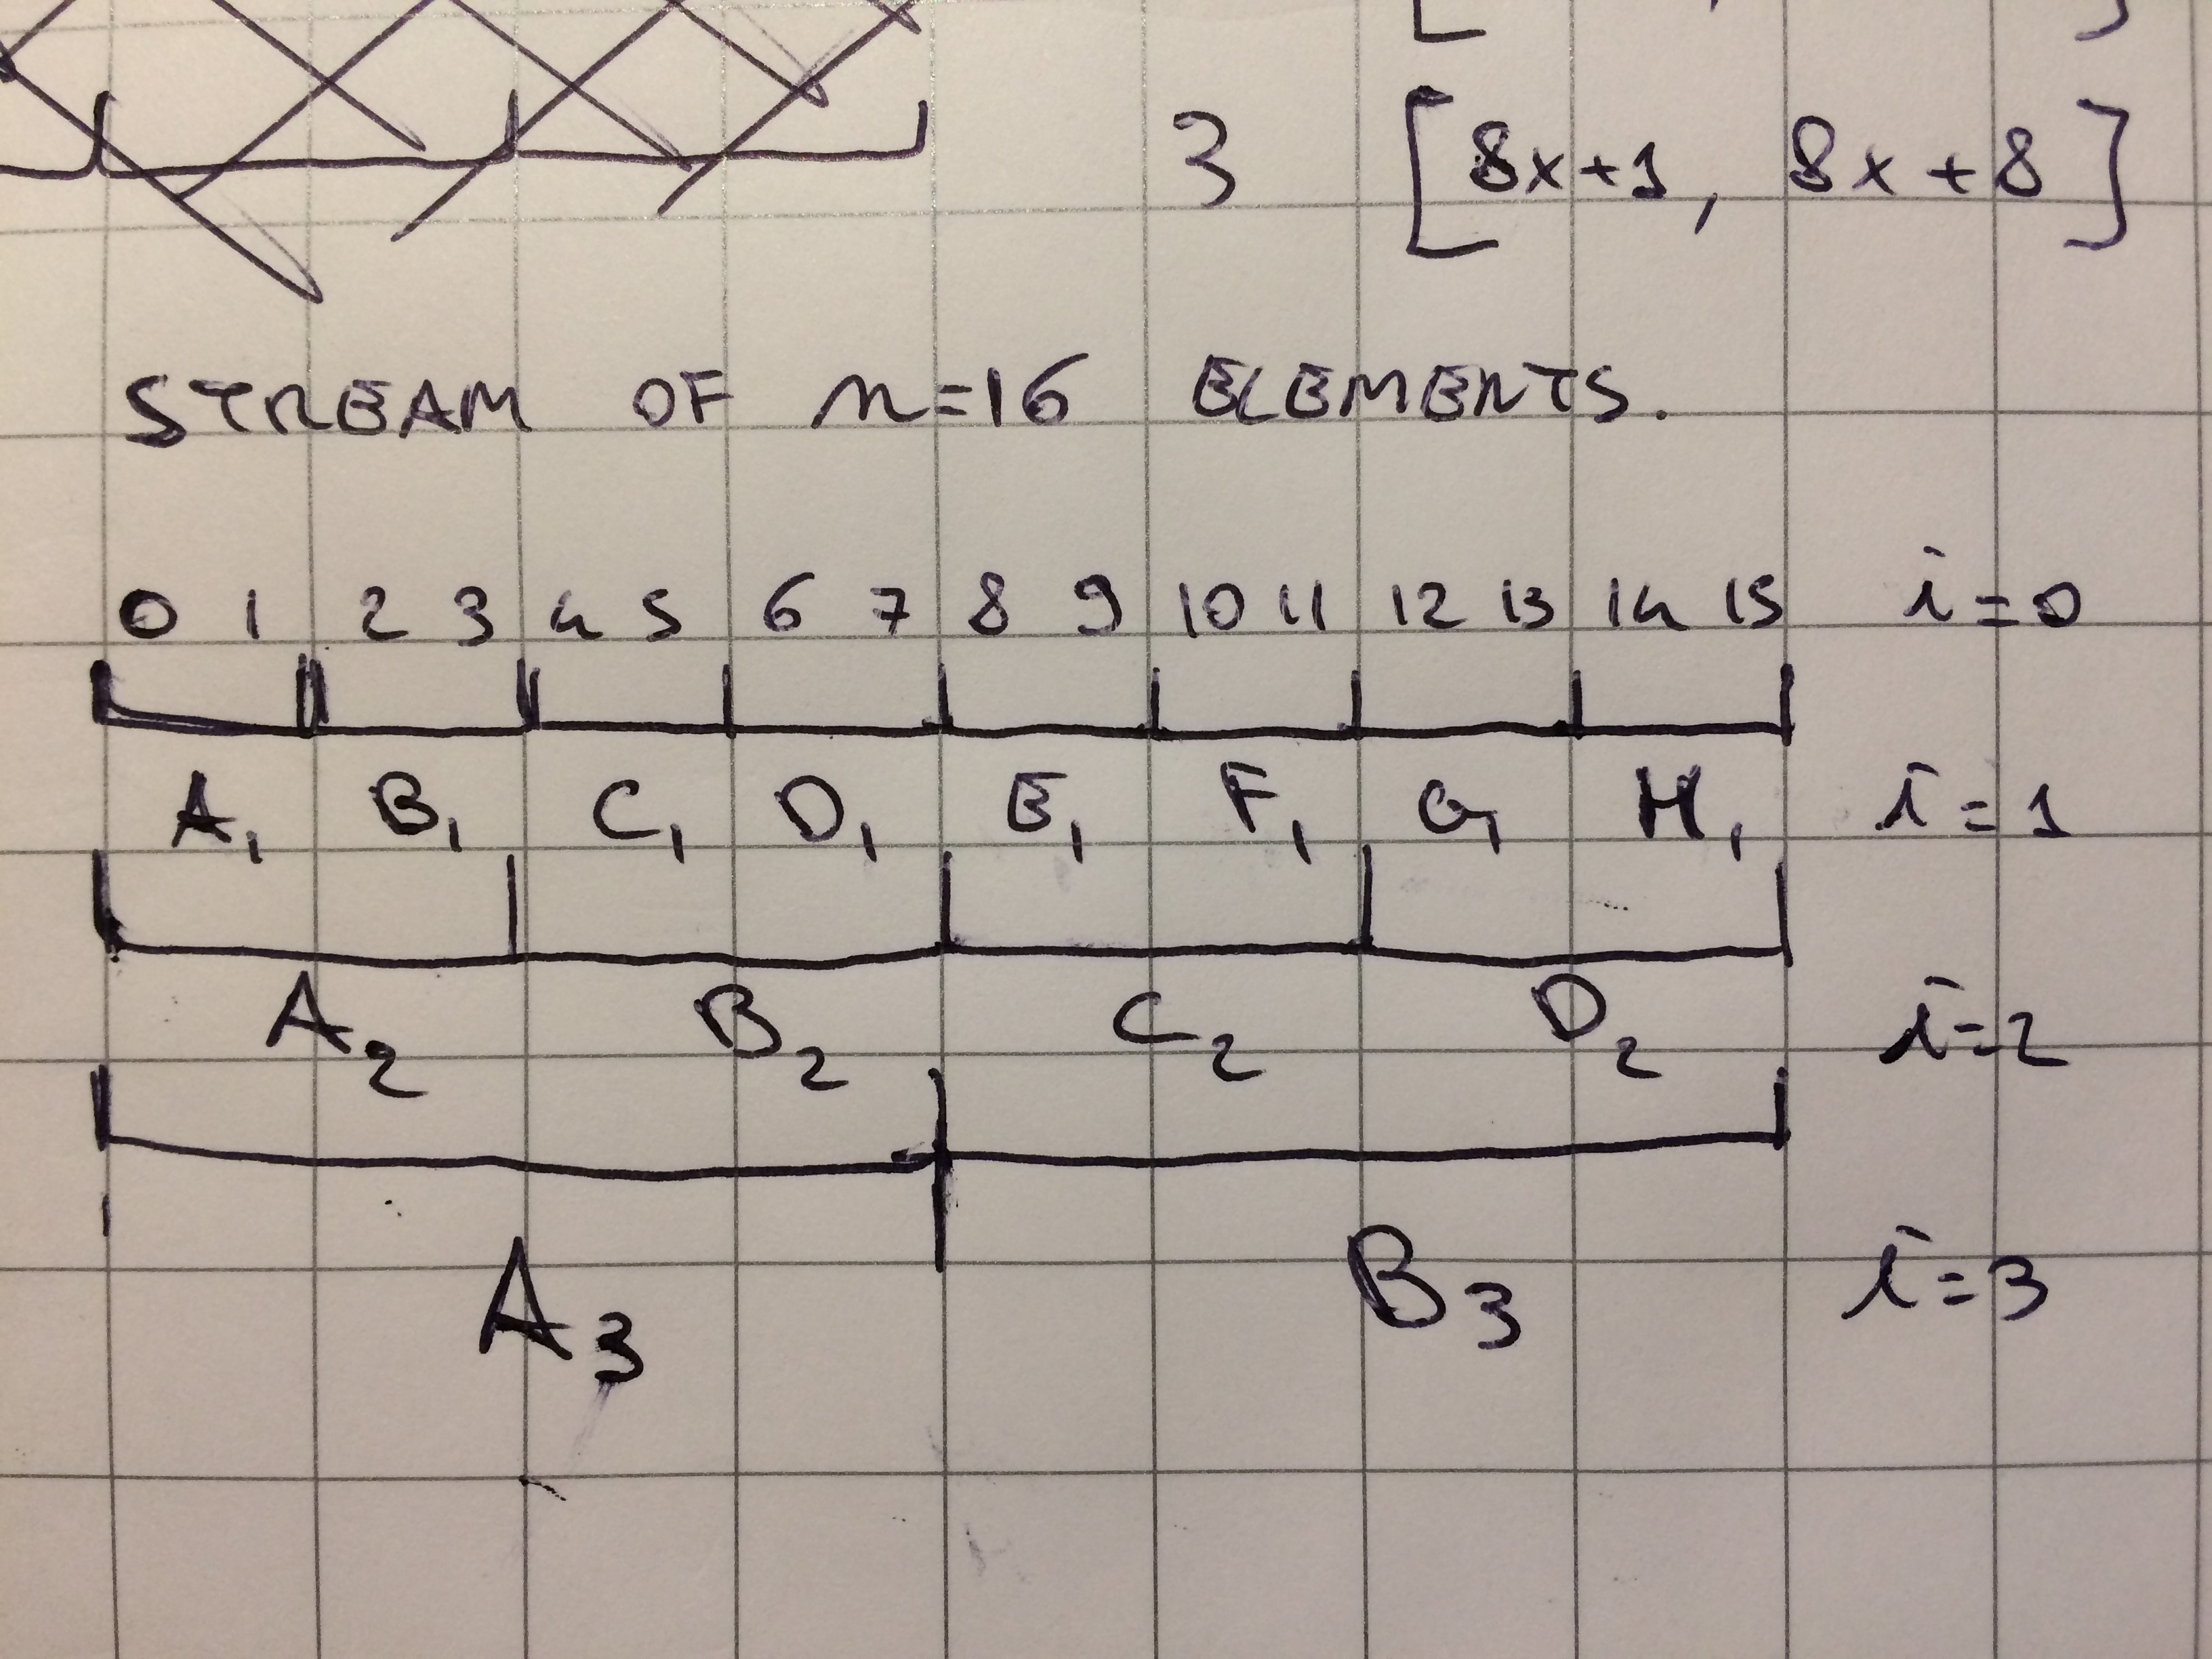
\includegraphics[scale=.1]{av_tree}\\
The sketch corresponding to ($i=3$) will count occurences of $A_3$ and $B_3$ (will count an $A_3$ every time a number in $\{0,1,2,3,4,5,6,7\}$ arrives, and a $B_3$ when a $\{8,9,10,11,12,13,14,15\}$ arrives.); the ($i=2$) sketch will count $A_2$,$ B_2$, $C_2$, $D_2$ and so on.
Then for each arbitrary interval $(a, b)$ we just need to sum the corresponding dyadic intervals that makes it. (e.g. if I receive a query for $(7, 13)$, then i can just sum up the occurences of $C_2$, $G_1$ and "$7$").\\\\
A count-min sketch table is kept for each set of dyadic intervals of length $2^i$, one for each level in the tree (one for each value of i). Thus we have $log_2 n$ vectors $\widetilde{F_i}$ and, in line of principle, $log_2 n$ vectors $F_i$.

You can see this as associating each new sketch to a reencoding of the original stream, where you have partitioned the alphabet in $2^i$ subsets of symbols and represented each of them with a single new symbol.
Say: ABCD as alphabet, map AB $\rightarrow$ E, CD $\rightarrow$ F; each time you witness A \emph{or} B you count an occurrence of E, each time you witness C \emph{or} D you count an occurrence of F.

Witnessing a new element in the stream will therefore trigger an update to all the $log_2 n$ tables.
\\
\\
The idea for a range query is to partition the range into dyadic intervals (of a number of sizes, in general, thus from a number of CMS tables) and return as result the sum of the values stored in the CMS tables for the corresponding intervals [see this \href{http://dimacs.rutgers.edu/~graham/pubs/papers/cm-full.pdf}{link} for further reference].
\\
\\
It can be shown\footnotemark that any range will be split at most into $2log_2 n$ dyadic intervals.

\footnotetext{First, note that:
\begin{itemize}
\item No three intervals of the same length can be contained in the partition of the same query, otherwise you could merge two of them;
\item If there are two consecutive intervals of the same length, they must belong to two different larger "parent" intervals (otherwise you could replace them with their parent), i.e. their union cannot belong to the dyadic partition.
\end{itemize}
Thus, there are at most 2 intervals of each possible size in the partition. As the sizes are $log_2n$ in all, the partition is made up of at most $2log_2n$ intervals.
}

Therefore for each query we access $t \leq 2\ log\ n$ counters $c_1,c_2,...,c_t$. We then, want to proof $Pr[\sum^t_{l=1}c_l > \sum^j_{k=i}F[k] + 2\epsilon\ log\ n ||F||]<\delta$.

Firstly, we notice that each counter $c_i$ represents an interval $[a,b]$ and it value is $\sum_{k=a}^b (F[k]) + X_i$, where $X_i$ is the rubbish of that particular interval. Then, give an interval $[l,r]$, and the counters we have $\sum^t_{i=1}c_i = \sum^r_{k=l}F[k] +X $, where X is the total error (notice that this works because the interval are disjoint). Then we substitute to the previous equation and we have:
\begin{align*}
Pr &[\sum^t_{l=1}c_l > \sum^r_{k=l}F[k] + 2\epsilon\ log\ n ||F||]<\delta \\
Pr &[ \sum^r_{k=l}F[k] +X  > \sum^r_{k=l}F[k] + 2\epsilon\ log\ n ||F||]<\delta \\
Pr &[ X  >  2\epsilon\ log\ n ||F||]<\delta \\
\end{align*}
Now, we apply Markov inequality and by the linearity of the expectation we have: $$Pr [ X  >  2\epsilon\ log\ n ||F||] \leq \frac{E[X]}{2\epsilon\ log\ n ||F||} \leq \frac{\sum_{i}^{2log_2(n)} E[X_i]}{2\epsilon\ log\ n ||F||}$$
\\
\\
Now, let $d(i)$ be the depth in the tree to which the dyadic interval $i$ belongs (identifying its CMS table). We see that $\forall i.E[X_i]< \frac{\epsilon}{e}||F_{d(i)}||_1$, but $\forall  x, y.||F_x||_1 = ||F_y||_1 = ||F||_1 \implies E[X_i]< \frac{\epsilon}{e}||F||_1$.

\noindent
(by definition $||A||_1 = \sum^n_{h=1}|A[h]|$, that is in our case we sum the frequencies of symbols, which sum up to the same total amount no matter how we group them with a reencoding)
\\
\\
Thus we have $$\frac{\sum_{i}^{2log_2(n)} E[X_i]}{2\epsilon\ log\ n ||F||} \leq \frac{2 \frac{\epsilon}{e}log \ n||F||}{2\epsilon\ log\ n ||F||}= \frac{1}{e}$$
This is the probability of error (that the sum of garbage is more the $2\epsilon\ log\ n ||F||$) in row $j$ (the min, potentially distinct for each table).
\\
\\
Since we choose the row of each table that minimize the sum of the counter (by definition), then there must be an error in all the row $r$. Thus we have $\frac{1}{e^r}=\delta$ since $r=ln(\frac{1}{\delta})$.\\ \\

A little example: suppose we have $n=16$ (item), then a range $[1 \dots 16]$. Thus, we query $(8,12)$, this interval is fully included, then we split in $[1 \dots 8]$ and $[9 \dots 16]$ (we go down in the tree). $[1 \dots 8]$ is still too big then we split in $[1 \dots 4]$ and $[5 \dots 8]$,  $[1 \dots 4]$ is not included then we take it off. $[5 \dots 8]$ for the same reason we split it in $[5 \dots 6]$ and $[7 \dots 8]$ and so on.\\
\end{document}